\noindent
% VJ: We had all of this above, I think
% AV : Accepted - Suggest we remove the complete document from the bigger document.

%\paragraph{The Smart Patient Health Record (SPHR) is the combination of a patient's data, and the patient's control over access to their data. By gathering together all of the data into a single source, we allow the patient to have direct control over who can see what.}

%\paragraph{Our stated our choice for database format is Data Vault. This is a highly flexible format that will allow for continuous changes to what is stored in them, future-proofing the underlying design of the SPHR.}

%\begin{figure}
%    \centering
%    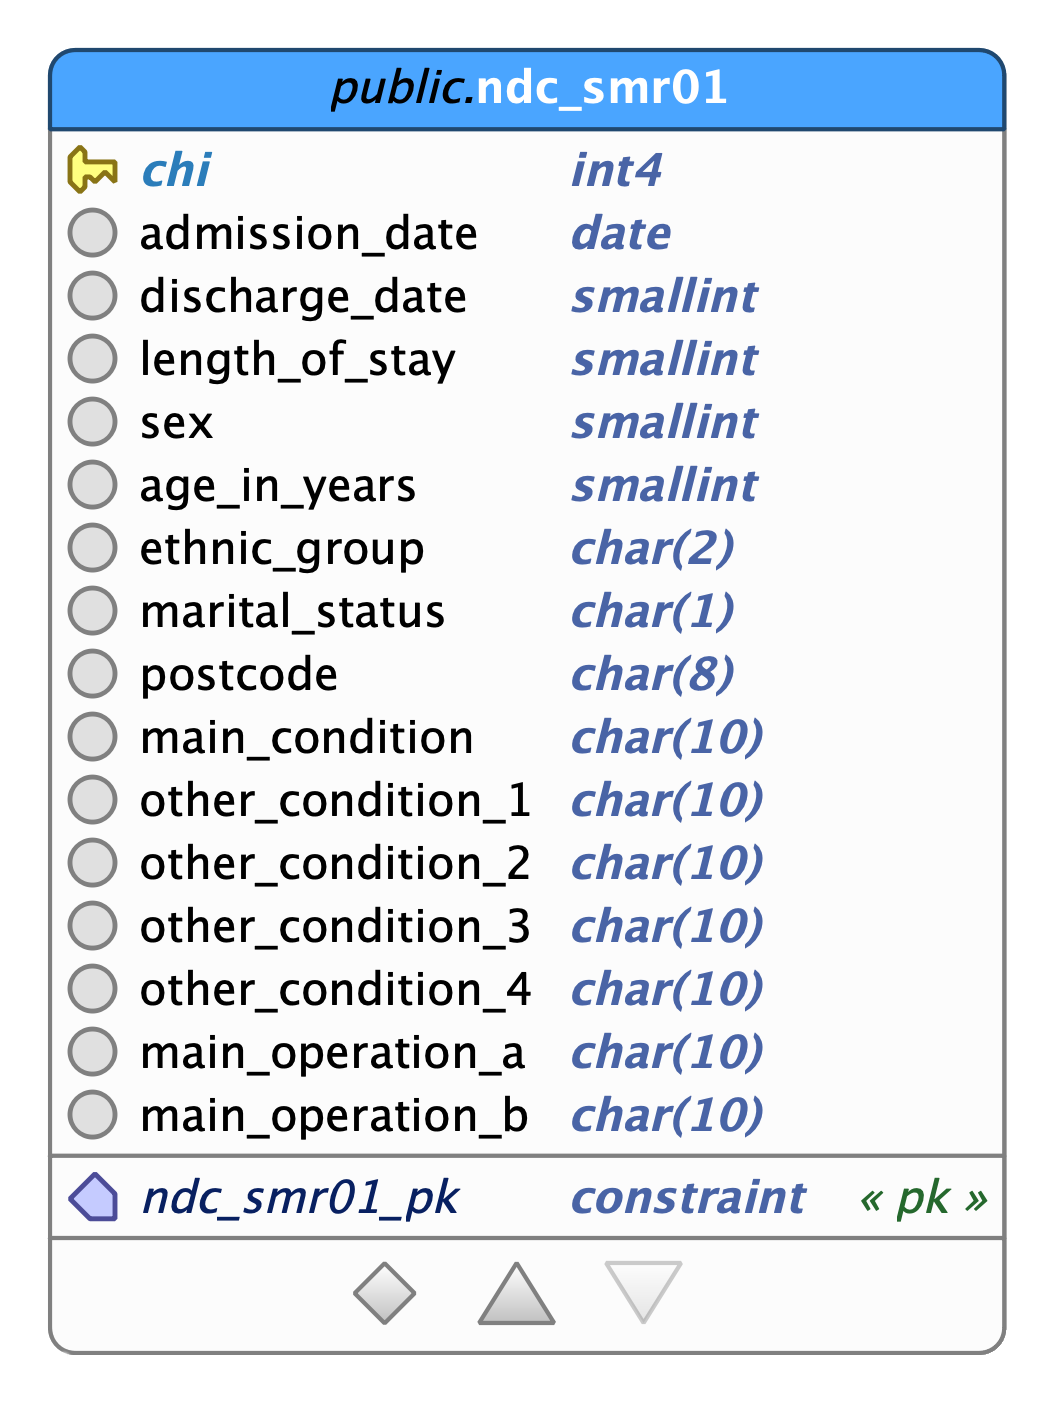
\includegraphics[width=45mm]{images/DataVault/smr01_source.png}
%    \caption{Example of source table}
%    \label{fig:smr01_source}
%\end{figure}


%\begin{figure}
 %   \centering
  %  \includegraphics[width=80mm]{images/DataVault/DataVault.pdf}
   % \caption{Example of source table abstracted into Data Vault}
    %\label{fig:dv_smr01}
%\end{figure}

%For example, Figure~\ref{fig:smr01_source} shows a part of the Edinburgh Cancer Gateway Centre use case, described in more detail in Section~\ref{sec:XX}. It contains information about one hospital visit of one patient. When abstracted into a data vault, the person hub would refer to patients, the time hub would refer to the dates and times of the hospital visits, and the object hub would contain the operations. The person hub contains the \emph{person demographic details} satellite, the time hub contains the \emph{admission date} satellite and the object hub contains the \emph{operations} and \emph{conditions} satellites (See Figure~\ref{fig:dv_smr01}).